% !TeX root = ../main.tex
% Add the above to each chapter to make compiling the PDF easier in some editors.

\chapter{Related Works}\label{chapter:related_works}


\section{Traditional Approaches for Prognostic and Health Management}

Traditionally, model-based and data-driven models were used as PHM systems. Model-based methods predict the health condition based on physical models, which describe the underlying mechanisms of degradation. Uncertainties in the machine processes as well as noise make the application of physical models difficult. Often, the identification of all model parameters is difficult and requires a lot of experiments. Data-driven methods learn a mapping relationship between the health condition state and monitoring data. Such methods do not use physical information about the degradation process. The performance of data-driven approaches highly depends on the quality and amount of the training data. Besides that, data-driven models might lack from generality. The models are just optimized to perform well on the working conditions which are present in the train data. Both, model-based and data-driven approaches suffer from different limitations \cite{DENG2020}. In the following, data-driven and model-based approaches in the context of PHM for BSDs are presented. 

\subsection{Model-Based Approach: Defect Frequency Estimation Based on a Model Simplification of Ball Screw Drives as Rolling Bearings}
Lee et al \cite{Lee2015} propose a diagnosis system, which in first place determines the characteristic frequencies for different machine defects. By filtering the machine signals for those defect frequencies, the type, severity and location of degradation signs in the machine can be predicted. Lee et al developed a test bed containing one BSD and linear motion guides. An accelerometer was mounted on the BSD nut measures vibrations. Holes with a diameter of 3 mm were punched in the BSD shaft to simulate the degradation. The ongoing process of fatigue was modeled by increasing the number of holes in the shaft. The motor was actuated with a constant velocity while the data was recorded.

Lee et al use a method, which was proposed by Harris and McCool \cite{Harris1996}, to estimate the characteristic defect frequencies. This method treats the BSD as a rolling bearing, where the screw shaft can be considered as inner and the nut as outer ring. From the construction details and the relative speed between the BSD components, the defect frequencies can be calculated. The ball pass frequencies of the shaft (BPFS) and nut (BPFN), as well as the ball spin frequency (BSF) are considered as defect frequency: 
\begin{equation}
    BPFS = \frac{1}{120}zn(1+\frac{D_{w}}{d_{m}}cos\alpha),
    \label{eq:defect_frequency}
\end{equation}
\begin{equation}
    BPFN = \frac{1}{120}zn(1-\frac{D_{w}}{d_{m}}cos\alpha),
\end{equation}
\begin{equation}
    BSF = \frac{1}{120}n\frac{d_{m}}{D_{w}} (1-\frac{D_{w}}{d_{m}}cos\alpha)(1+\frac{D_{w}}{d_{m}}cos\alpha) ,
\end{equation}
where $\alpha$ is the contact angle between the ball, nuts and screw shaft, $d_{m}$ is the pitch diameter of the balls, $D_{w}$ is the diameter of a single ball, the rotational speeds of external and internal races are defined by $n_{e}$ and $n_{i}$ and $z$ is the number of steel balls. A more detailed visualization of the bearing parameters is shown in fig. \ref{fig:defect_frequency_calc}. 

\begin{figure}[H]
  \centering
  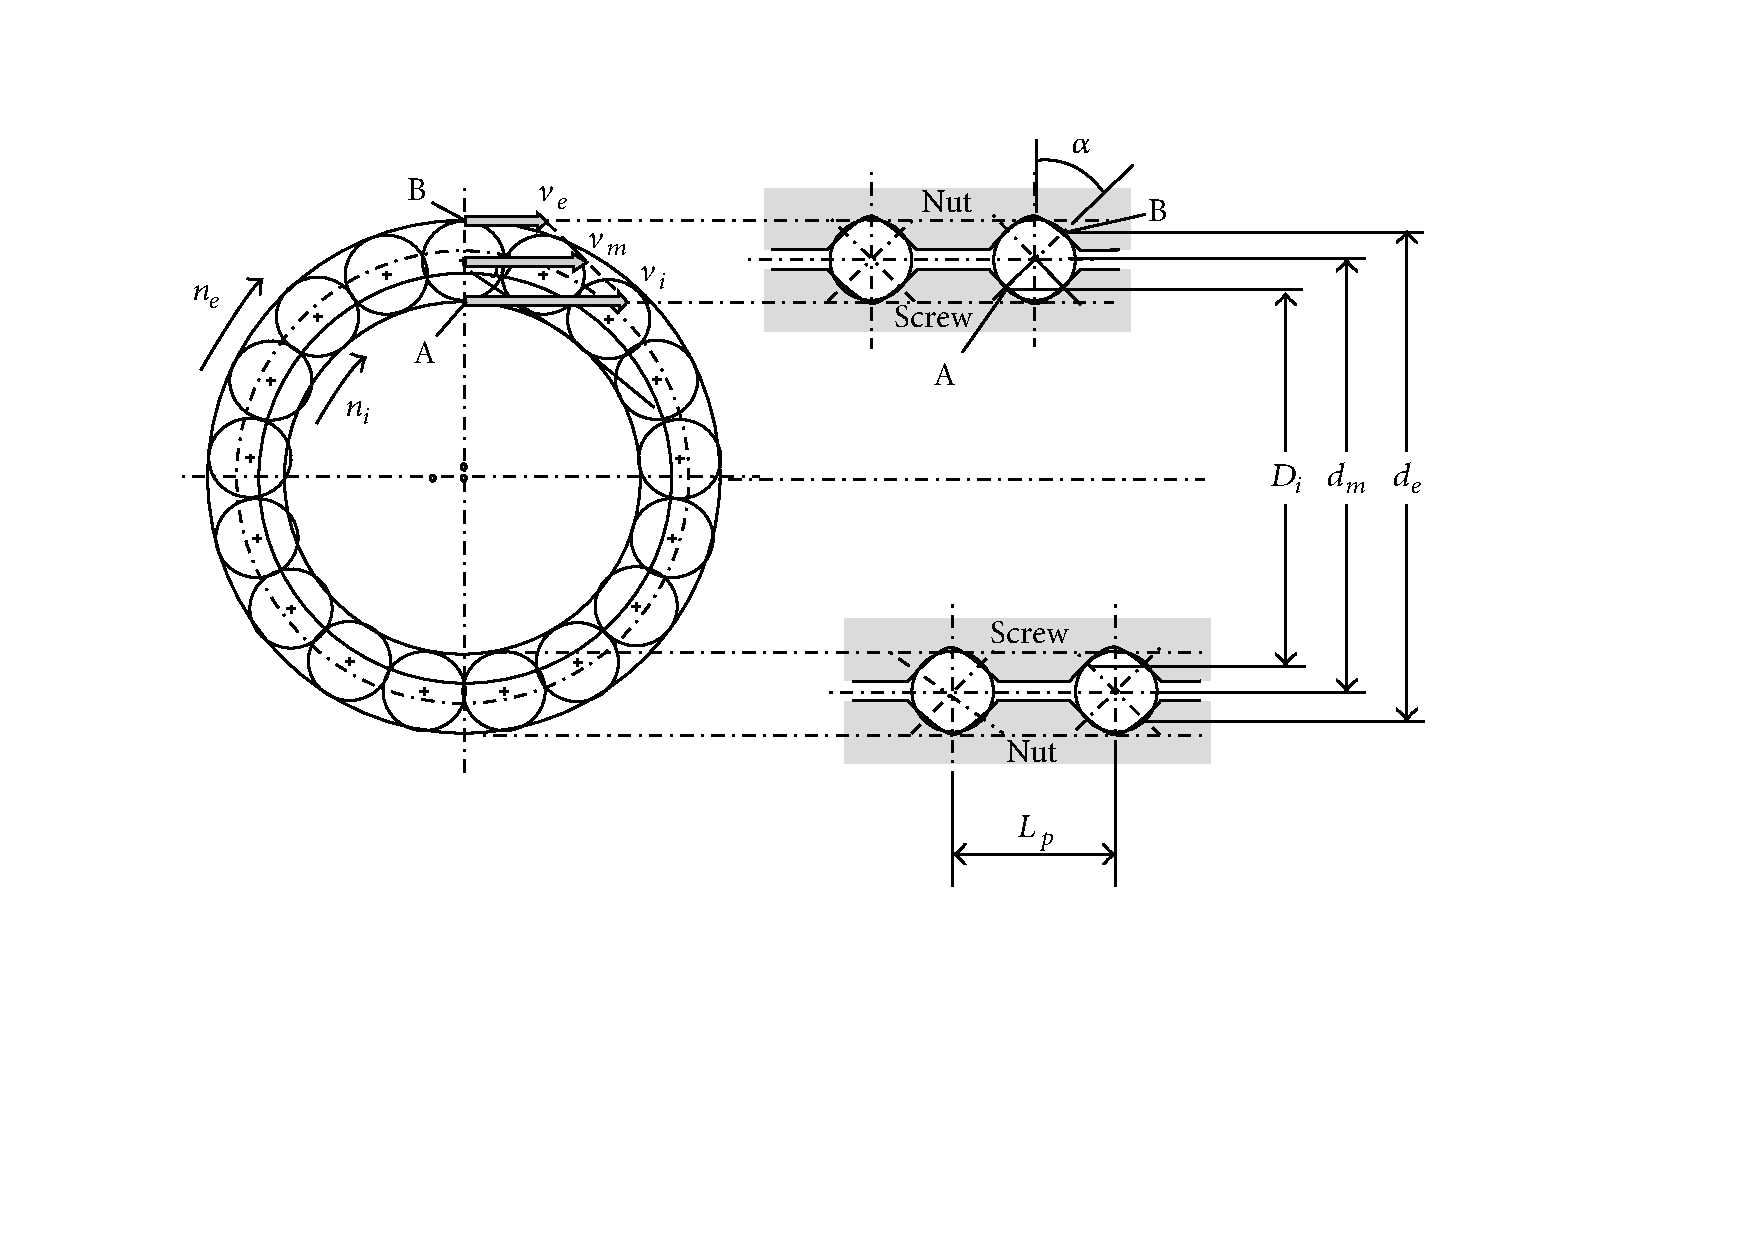
\includegraphics[width=.6\textwidth]{models_state_of_the_art/defect_frequency_calc.pdf}
  \caption{Simplification of BSDs as bearings for frequency calculation \cite{Lee2015}}
  \label{fig:defect_frequency_calc}
\end{figure}

The above derived frequencies are valid for bearings. To apply those to BSDs one has to replace $z$ and $d_{m}$ by the effective number of steel balls $z^{'}$ and effective pitch parameter $d_{m}^{'}$, which are defined as following:

\begin{equation}
    d_{m}^{'} = (L_{p}^{2}+(\pi D_{b})^{2})^{\frac{1}{2}},
\end{equation}
\begin{equation}
    z^{'} = \frac{d_{m}^{'}}{D_{w}}.
\end{equation}
The translation between the regular and effective parameters is visualized in fig. \ref{fig:defect_frequency_transfer}. 

\begin{figure}[H]
  \centering
  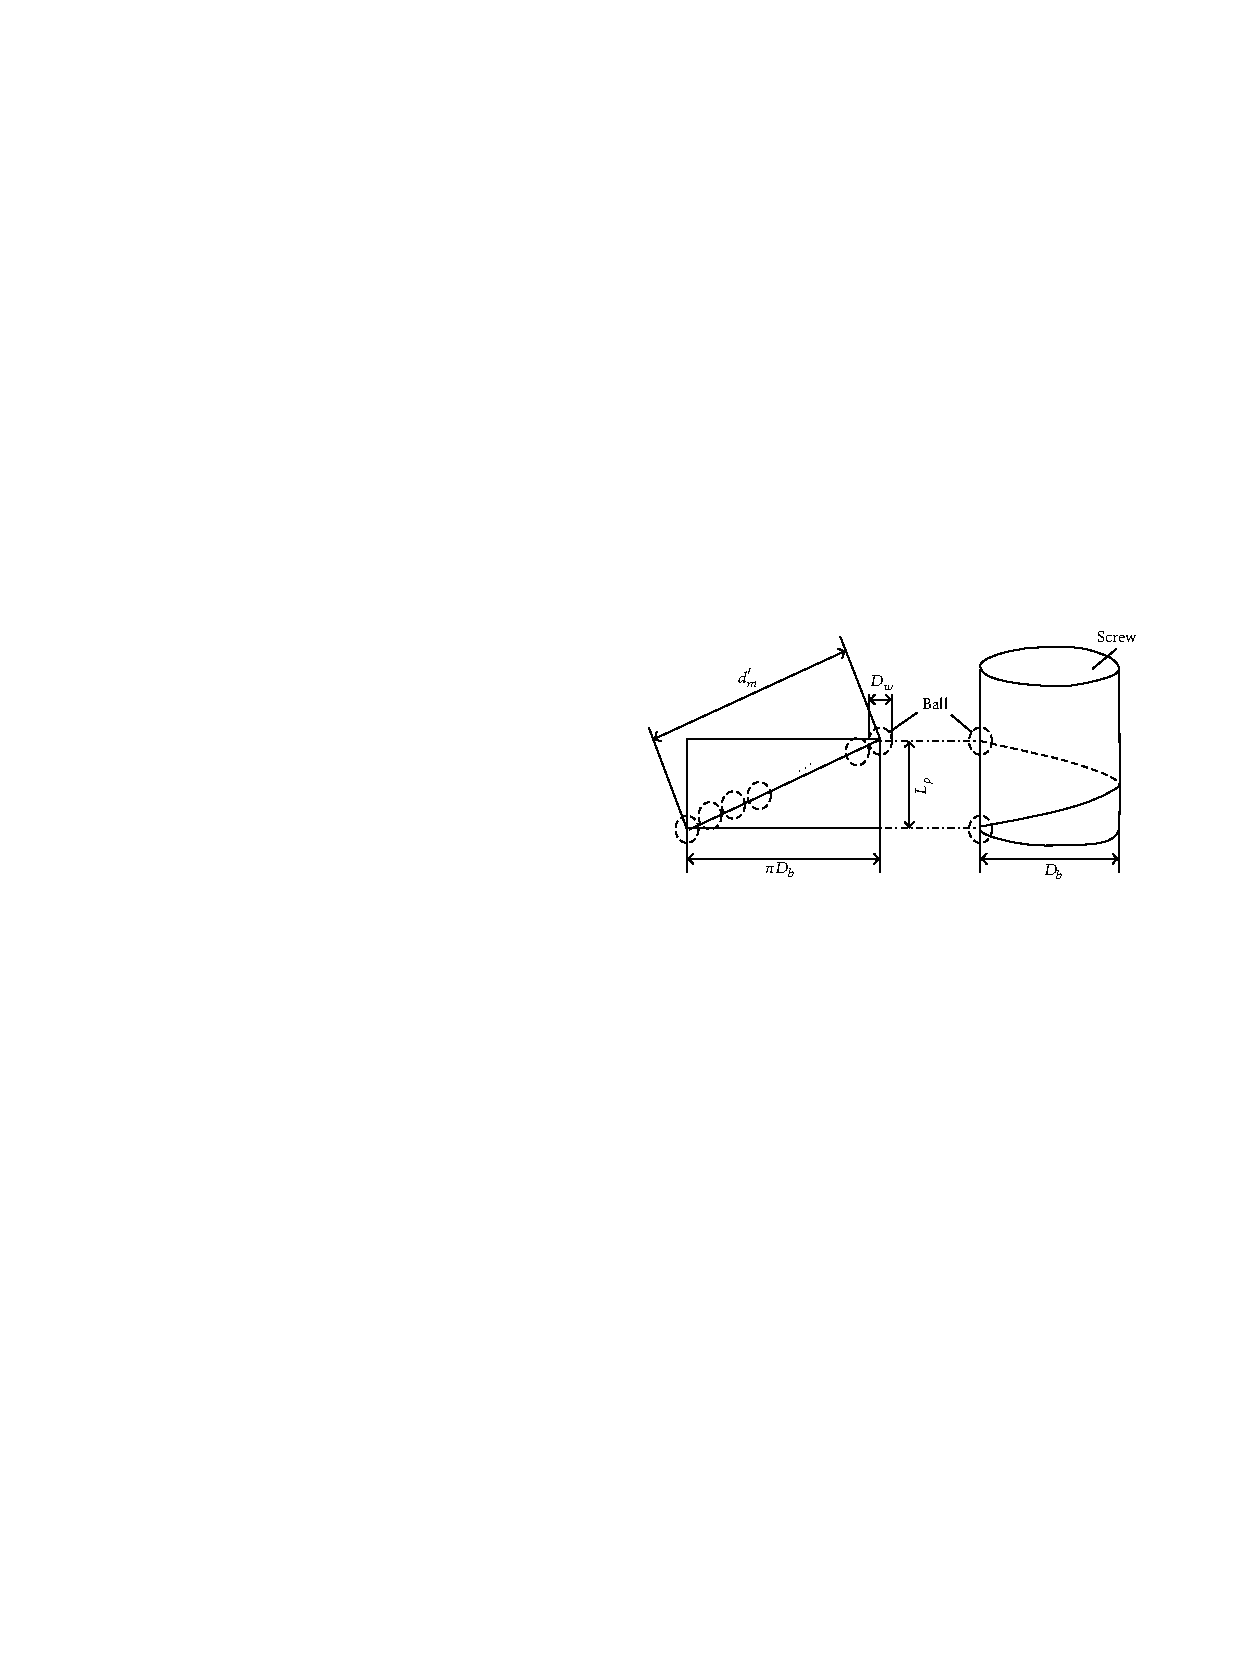
\includegraphics[width=.7\textwidth]{models_state_of_the_art/defect_frequency_transfer.pdf}
  \caption{Transfering pitch parameter and number of steel balls from bearings to BSDs \cite{Lee2015}}
  \label{fig:defect_frequency_transfer}
\end{figure}

Li et al identified the BPFS frequency as the most expressive and reliable one for supervising the health condition of BSDs. To calculate the BPFS for ball screw drives the equation \ref{eq:defect_frequency} must be combined with the effective pitch parameter $d_{m}^{'}$ and effective number of steel balls $z^{'}$. The wavelet transform (Daubechies Wavelet (db14) function) is used to transform the machine signals in the two-dimensional time-frequency domain. Each time the steel balls of the BSD pass a whole in the surface of the BSD shaft, the machine signal shows a corresponding defect pattern. This time-related information are an indicator for detect location. The frequency-related information provide information about the severity and type of degradation. Fig. \ref{fig:defect_frequency_model} visualizes the proposed approach during testing.

\begin{figure}[H]
  \centering
  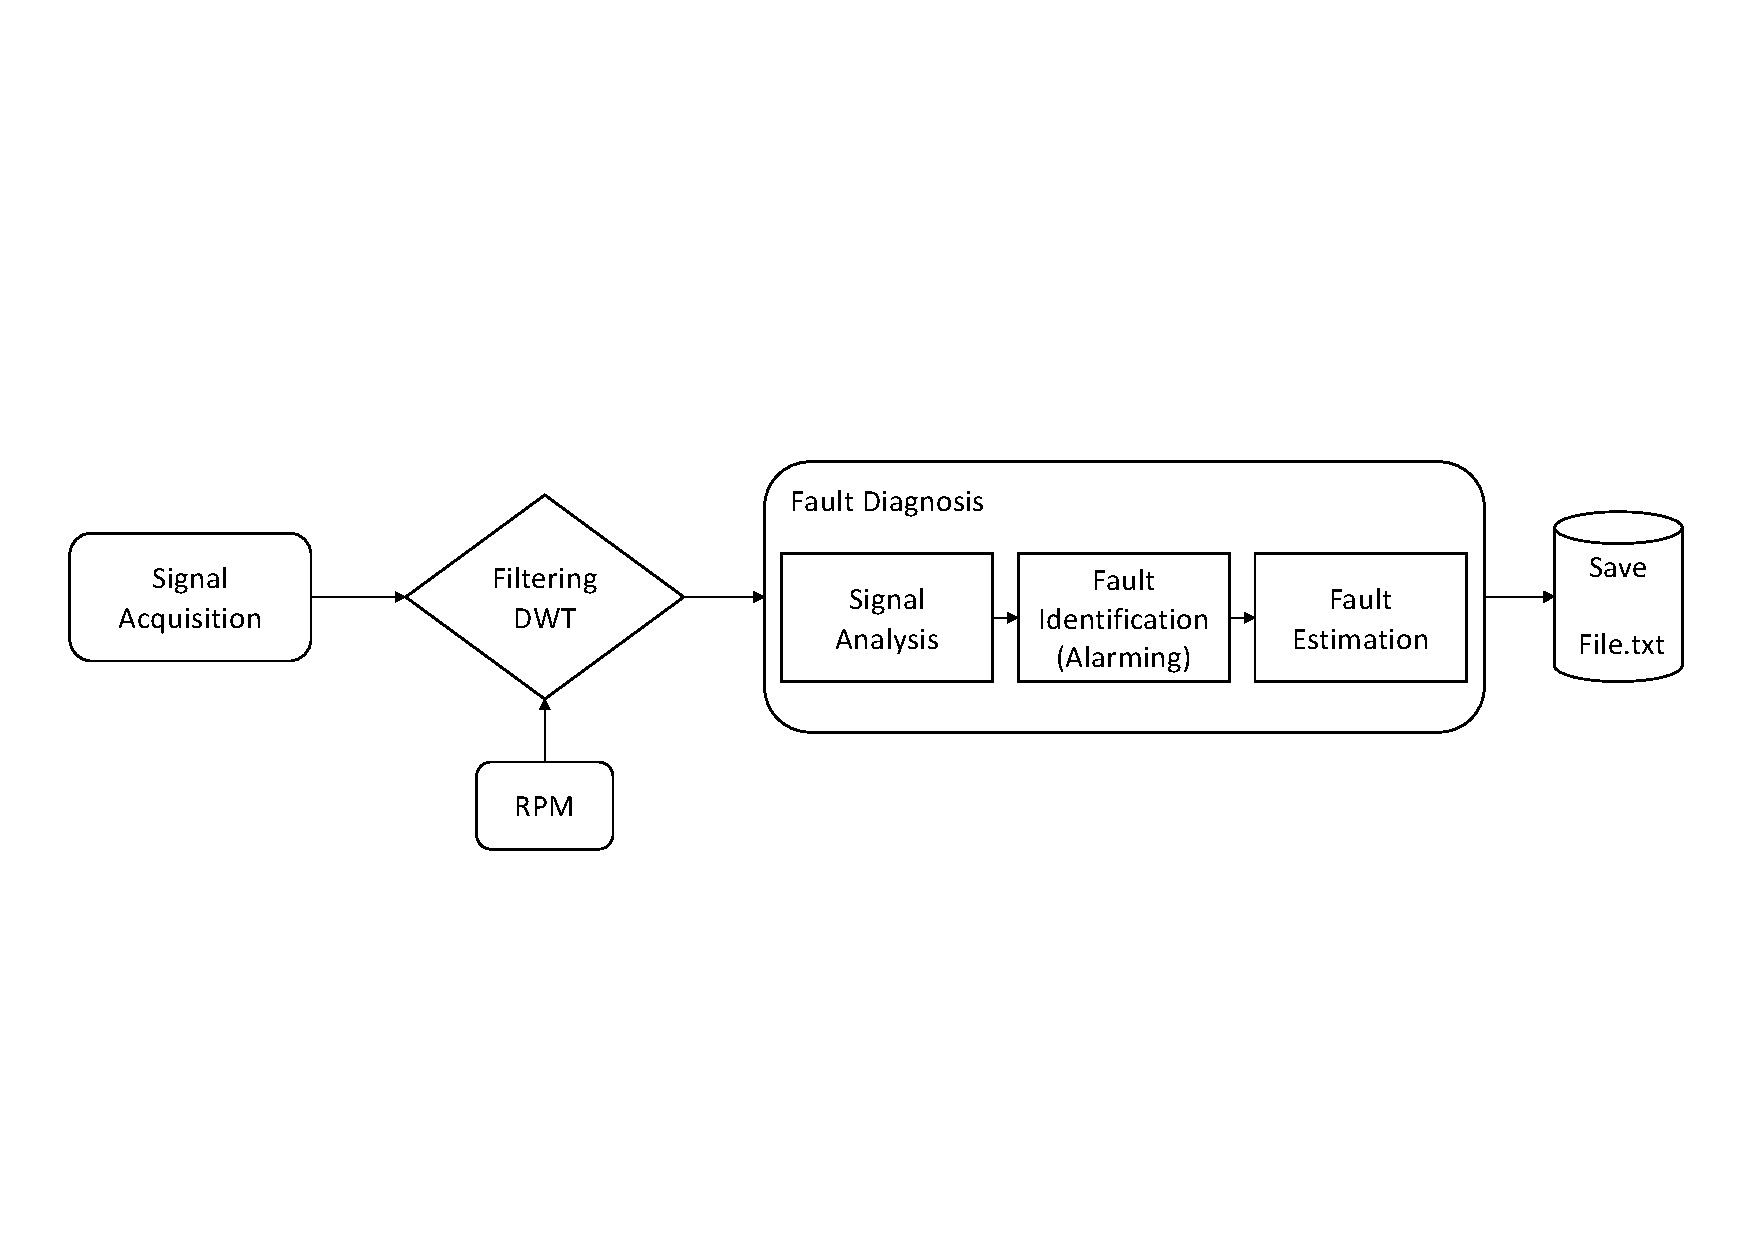
\includegraphics[width=.95\textwidth]{models_state_of_the_art/defect_frequency_model.pdf}
  \caption{Failure diagnosis system by calculating defect frequencies based on \cite{Lee2015}}
  \label{fig:defect_frequency_model}
\end{figure}

\subsubsection{Conclusion}
Lee et al. assume that defects and degradation are mainly subjected to rolling friction. Often times such simplifying assumptions are made when developing model-based PHM systems. In reality the balls in BSDs are rotating, revolving, and sliding, which might create a highly complex degradation process which will be hard to modeled accurately. When applying data-driven PHM systems one can define the degradation classes individually by labeling the recorded dataset accordingly. Lee et al. have to stick to the definitions set by Harris et al. \cite{Harris1996}, when they defined defect frequencies corresponding to specific physical degradation mechanisms in rolling bearings. When searching machine signals for the specific defect frequencies Lee et al. came across other distinct frequencies coming from major electrical noise. Lee et al. just tested their approach on a small testbed. When applying that approach on real-world machines, a lot of other components might influence the characteristic defect frequencies. Finding all parameters to calculate the defect frequencies might require a lot of effort in measuring and testing. Often these parameters are assumed to be constant throughout the lifetime of the BSD. The rolling diameter for example will be reduced thoughout the lifetime of a rolling bearing. Anhow, this parameter is used as a constant parameter in the calculation of the defect frequencies for rolling bearings. When transfering the calculated defect frequencies from the rolling bearing to the BSD only structural differences are considered. Lee et al. completely ignore the linear movement, which differs the function of rolling bearings and BSDs fundamentally. Lee et al. simulated the degradation process by punching holes with a diameter of 3 mm on the grooves of the BSD shaft. Solely the number of holes, but not their size does change during the simulation of the degradation. It is questionable whether this method simulates the degradation apropriately.  


-major electrical noise of frequency, 60 Hz, has been cut off but its second harmonic, 120 Hz, was not filtered out
-system must run in steady state during evaluation in a rebuild test bed not an actual machine. Other machine parts can also influence the vibration. The vibration of other machine parts should be filtered out from the recorded the data
-Autar identified that defects such as fatigue, fractures, and strains are mostly found in the parts that are subject to rolling friction. Modeling of degradation restricted to rolling friction. balls are rotating, revolving, and sliding in the inner and outer races. The defects occurring in screw shafts and steel balls represent major failure modes. But those are not the only defects and failure modes. Very limited view on the degradation process.
-difficult measuring of all the parameters used in the model
-holes with a diameter of 3 mm were punched on the ball groove with a carbide drill to simulate the defects --> no real degradation scenario
The progressing degradation is just modeled by the number of holes and not the scale of the individual holes
-rolling diameter is continously reduced throughout the operation but used as fixed value in the formulas (cite Denkena)
-the transformation of the defect frequencies from rolling bearing to BSD just considers structural differences. Anyhow, there are also big differences in the application of the two components. The linear motion in BSDs will most certainly also influence the 
- is restricted to fault types which are defined by the defect frequencies. Amplitude is used as indictor for degradation state --> interpolation between max and min frequency is diffcult

\subsection{Data-Driven Approach: Principal Component Analysis based Sensor Fusion of Multiple Statistical Features}

Denkena et al \cite{Denkena2021} present a method to monitor the degradation of BSDs. Firstly, several hand-crafted statistical features are extracted from the machine signals. Afterwards, a sensor fusion approach based on principal component analysis is used to combine those features. In the end, decision trees solve the classification task. A test bed consisting of a single BSD was used to evaluate the proposed approach. Internal control signals were provided by the internal controller and three uniaxial acceleration sensors measure vibrations in the system. The machine data was recorded during constant feed rate over the whole length of the test bench. The proposed PHM method can be separated in four steps:

\begin{itemize}
    \item [\textbf{Data acquisition:}] The method processes vibration signals from three uniaxial acceleration sensors as well as internal control signals simultaneously. The signals are concatenated, synchronized and separated in phases of zero acceleration (constant movement of nut on the shaft) and non-zero acceleration (direction change movement at each end of the BSD shaft). The ball screw was moved over the length of the test bench with various feed rates (6000 mm/min, 11000 mm/min, 17000 mm/min,20000 mm/min) \cite{Denkena2021}.
    \item [\textbf{Feature extraction:}] Information about the preload classes are extracted through statistical features (e.g. kurtosis, median, impulse factor, ...). The features are extracted for each signal and segment. Each feature is evaluated by its robustness and statistical significance. The robustness is measured by the feature's dispersion around the median. After normalizing the feature with the z-score, the significance is investigated by the f-statistics.
    
    \begin{equation}
        \textbf{Z-score:}\qquad \tilde{x}_{i,j} = \frac{x_{i,j} - \bar x_{i}}{\sigma_{i}},
    \end{equation}
    
    \begin{equation}
        \textbf{F-statistic:}\qquad f = \frac{\sum_{j=1}^{J} i \cdot (\bar x_{j} -\bar x)^{2}/(J-1)}{\sum_{j=1}^{J} \sum_{i=1}^{I} i \cdot (\bar x_{j,i} -\bar x_{j})^{2}/(J \cdot (I-1))},
    \end{equation}
    where ${x}_{i,j}$ denotes the feature value j of a sample of class i, $\bar{x}_{i}$ is the feature mean value of class i, ${s}_{i}$ is the feature standard deviation of class i and $\bar{x}$ is the overall feature and class mean value, I and J is the number of all classes and features. Denkena et al see features as eligible for the diagnosing system if the dispersion around the median is smaller than $\pm$ 10 and the f-statistics is higher than a critical value of 10. The selected features are merged with the goal of maintaining the robustness and increasing the f-statistics  \cite{Denkena2021}. 
    
    \item [\textbf{Principal Component Ananylsis:}] 
    Principal component analysis (PCA) is a method to reduce the dimensionality of a data while retaining most of the information. Principle components are the directions in the feature space, along which the variation of the data is maximal. Using just a few principal components, each sample can be represented by a few number of variables \cite{Ringner2008}.
    
    \item [\textbf{Classification:}] Denkena et al decided to use a decision trees to predict a preload class based on the extracted features. Due to its low classification effort and good traceability, decision trees seem suitable for the classification task. For each signal and segment, a separate decision tree is used  \cite{Denkena2021}. 
\end{itemize}

\subsubsection{Conclusion}
In order to find features which work well for predicting the degradation state of BSDs, Denkena et al. extracted 1500 features for each signal segment. The suitability of the features differed for the working conditions, classes and signals. For feed rates higher than 11000 mm/min, the acceleration signals are not able to classify the preload classes accurately. The univariate features MAX, RMS and CRE can only separate some of the defined preload class. For changing preloads the features do not show a steady behaviour. When applying the features MAX and RMS on the acceleration signals, they increase from C3 through C2 to C1, but decrease towards C0. Linear interpolation can not be used to estimate the degradation state based on the feature values. For slower feed rates the features show better classification performance, but the inspection time increases as well. Finding a set of features which predict all BSD preload classes correctly while showing a steady behaviour, involves a lot of effort. These features just work reliably for specific signals and BSD working conditions. When redefining the preload classes or changing the working conditions or signals the whole analysis has to be repeated to reestablish a PHM system. To simulate the preload loss throughout the lifetime of BSDs, ball sets with different oversize were installed in the BSD. The physical degradation of the shaft the balls is neglected in the experiments.

\section{Domain Adaptation Approaches for Prognostic and Health Management of Ball Screw Drives}
In recent years, more and more intelligent and adaptive data-driven approaches were proposed for monitoring the health status of industrial machines. Especially in the computer vision community, domain adaption and transfer learning became a hot topic. Slowly models, developed in the computer vision context, also make its way in the PHM field. In the following, deep learning-based domain adaption approaches are presented for predicting the degradation status of BSDs and rolling bearings. Similarly to the method proposed in this thesis, the presented models are optimized to reduce the domain discrepancy measured by the MMD metric.

\subsection{Deep Domain Adaption based on MMD-Loss Deep Distance Metric Learning}
A PHM algorithm for rolling bearings, which optimizes the inter- and intra-class distance in the latent feature space and reduces the domain discrepancy with a MMD-loss, is presented by Li et al \cite{Li2018}. As visualized in fig. \ref{fig:Deep_distance_metric_learning_model}, the model proposed by Li et al contains a CNN and a consecutive classifier. In a preprocessing step, a FFT transform is applied to represent the raw vibration signals in the time-frequency domain. Max-pooling layers are included to reduce the model size. Batch-normalization layers reduce the internal covariate shift by normalizing the input distributions of the hidden layers. To prevent overfitting, dropout layers with a rate of 0.5 are included. The proposed method was evaluated on a rolling bearing dataset provided by the Bearing Data Center of Case Western Reserve University. The domain shift was generated by using testing data, which was exposed to additional environmental noise, and collected under a different working conditions than the source data. 10 health conditions with different fault location and fault size were defined. 

\begin{figure}[H]
  \centering
  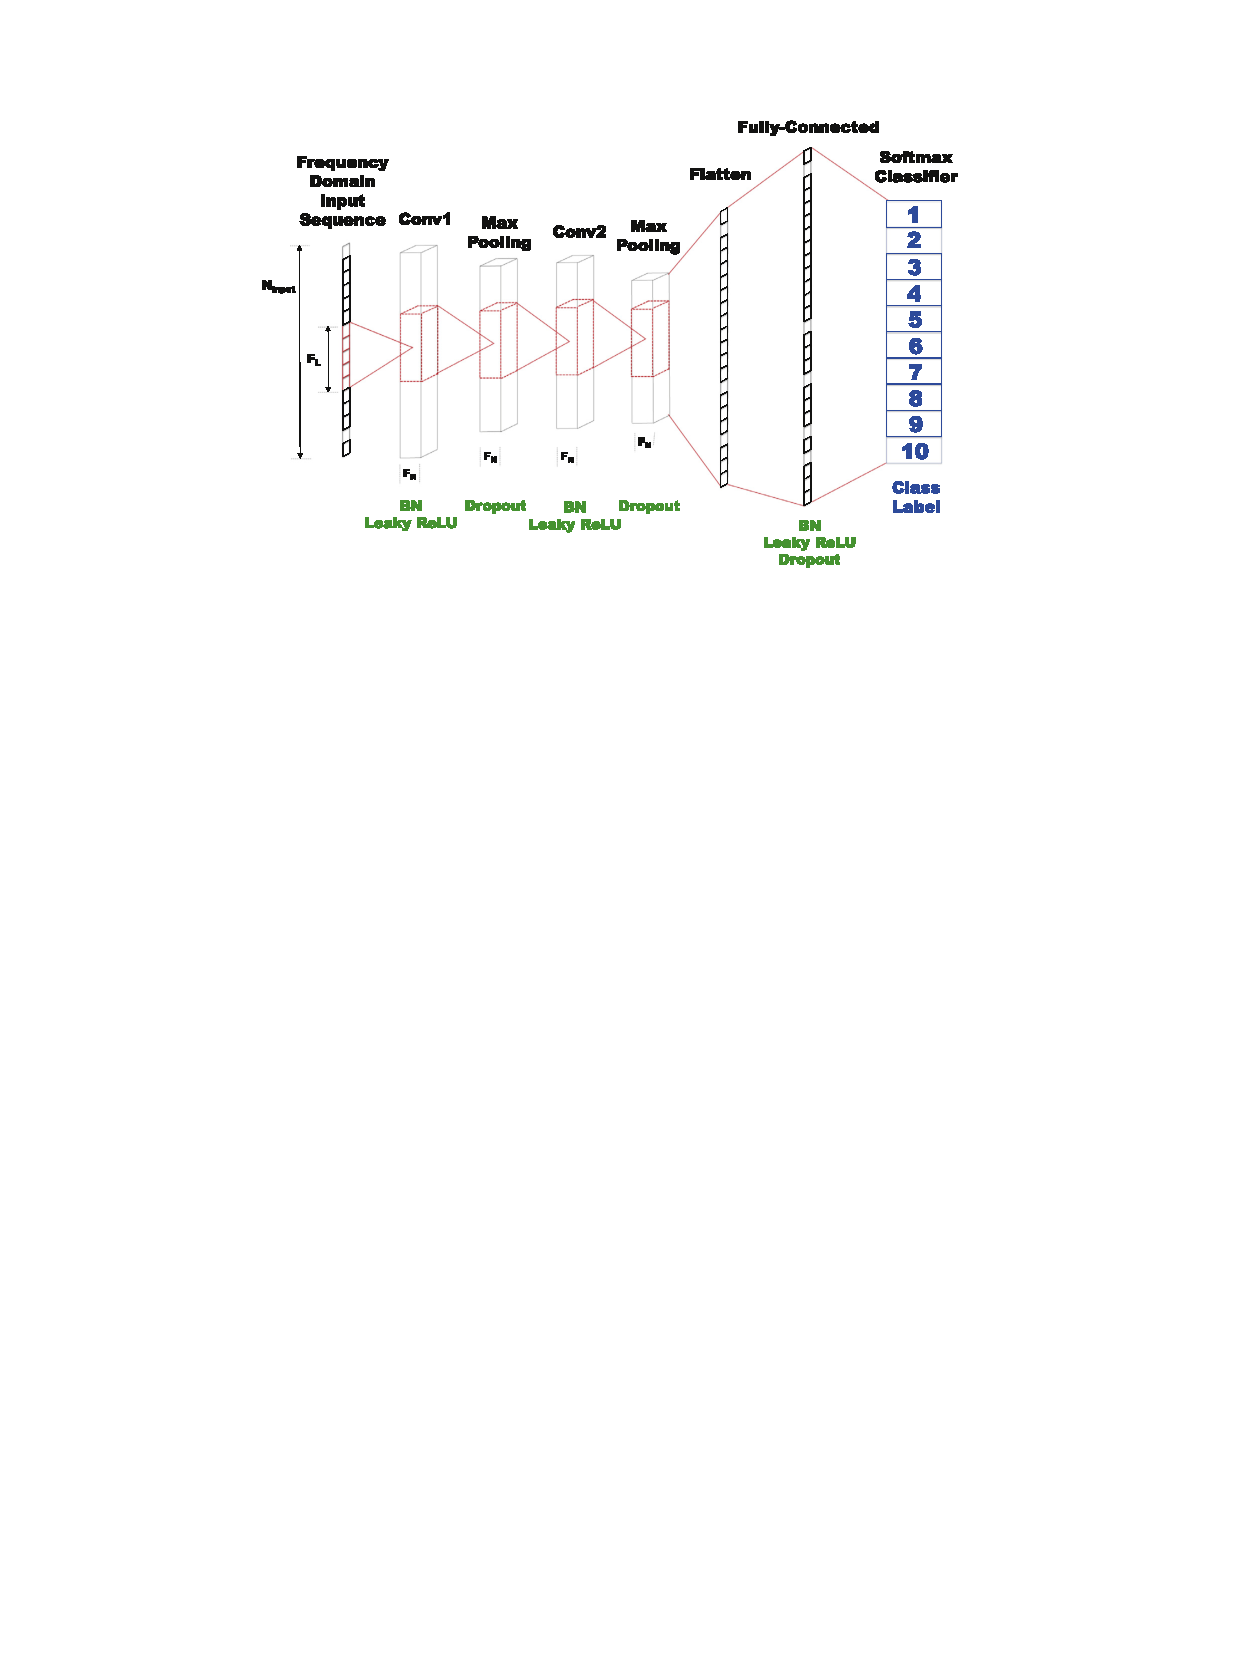
\includegraphics[width=.75\textwidth]{models_state_of_the_art/Deep_distance_metric_learning_model.pdf}
  \caption{Deep distance metric learning architecture proposed by Li et al \cite{Li2018}}
  \label{fig:Deep_distance_metric_learning_model}
\end{figure}

Li et al suggest to optimize the model such that the distance between source samples is minimized if they belong to the same class and maximized otherwise. This increases the separability and compactness of the classes, which makes the algorithm more robust against environmental noise. In order to calculate the intra- and inter-class distances the expectation and variance of source domain samples belonging to the same class is measured in the feature maps:

\begin{equation}
    \begin{aligned}
       &D_{inter} = |E[f^{(m)}x^{(i)}]-E[f^{(m)}x^{(j)}]|_{2}-\sqrt{Var[f^{(m)}x^{(i)}]}-\sqrt{Var[f^{(m)}x^{(j)}]}\\
       &D_{intra} = 
        \sum_{i=1}^{N_{class}} \sqrt{Var[x^{(i)}]},
    \end{aligned}
\end{equation}

where $N_{class}$ is the number of classes, $x^{(k)}$ denotes the raw input sample of class k, $f^{(m)}x^{(k)}$ denotes the feature representation of this sample in the m-th layer and $E[f^{(m)}x^{(i)}]$ and $Var[f^{(m)}x^{(i)}]$ are the corresponding expectation and variance. The inter- and intra-class distance are optimized with the following loss: $J_{Cluster} = - D_{inter} + \eta D_{intra}$. Since $J_{Cluster}$ requires the sample's labels, the optimization is restricted to the source domain. In addition to the distance metric learning the domain discrepancy is reduced by an MMD-loss in several FC layers. Lastly, a CE-loss in the final layer optimizes the network to classify the source samples correctly. In total, the network is optimized with the following weighted average of losses: 

\begin{equation}
    \begin{aligned}
    J_{total} = \alpha J_{Cluster} + \beta J_{MMD} + \gamma J_{CE}, 
    \end{aligned}
\end{equation}
where $J_{Cluster}$ is the loss optimizing the distances between the source domain samples, $J_{MMD}$ the MMD-loss,  $J_{CE}$ the CE-loss and $\alpha$, $\beta$ and $\gamma$ are the weights for calculating the weighted average \cite{Li2018}.



\subsection{Deep Domain Adaption based on MMD-Loss}
Azamfar et al \cite{AZAMFAR2020103932} proposed a deep learning-based domain adaption approach for PHM of BSDs, using a MMD-loss. An experimental test rig was build, containing a single horizontal guideway and a BSD, which were both fixed on a concrete base. Three accelerometers were installed to measure vibrations in X and Y directions. These sensors were mounted on the BSD nut and the bottom and top attachments of the BSD shaft. A sound pressure sensor captured the acoustic level when running experiments on the test rig. The torque and speed signals were acquired from the controller. In the experiments the guideways and BSDs were available in three different degradation classes. In the "normal" class the concerned component was operating normally, in the "faulty level 1" class it was deviating from the healthy condition and in the "faulty level 2" class it had to be replaced or repaired. In total nine different combinations of guideways and BSDs with different levels of degradation were combined. Azamfar et al acquired data by performing a full cycle of BSD operation, which contains two full forward and backward movements along the guideways. The data from each recording was split in phases with constant (forward, backward movement) and changing BSD nut velocity (turning point at the end of BSD shaft). The training was restricted to the signals recorded during the phases with constant speed, which were fed to the model as a single input without any windowing. The data dimension was reduced by a simple down-sampling method. The full cycle of BSD operation was recorded with different BSD velocities (200, 400 and 600 mm/s). The data distribution discrepancy in the recordings with different BSD velocities created am domain shift. The proposed method was evaluated on a 9 class classification task, including all combinations of BSD and guideway degradation classes. The proposed neural network architecture is presented in fig. \ref{fig:Azamfar_model}. It contains a feature extractor of four alternating one-dimensional convolutional and max-pooling layers and a subsequent classifier. To prevent overfitting, the dropout layers with the rate of 0.3 are included. The ReLU activation function is used throughout the network. The proposed model optimization includes a source CE-loss to improve the classification accuracy on the source domain data. Besides that the domain discrepancy is reduced by a MMD loss, which is applied in the penultimate fully connected layer. 

\begin{figure}[H]
  \centering
  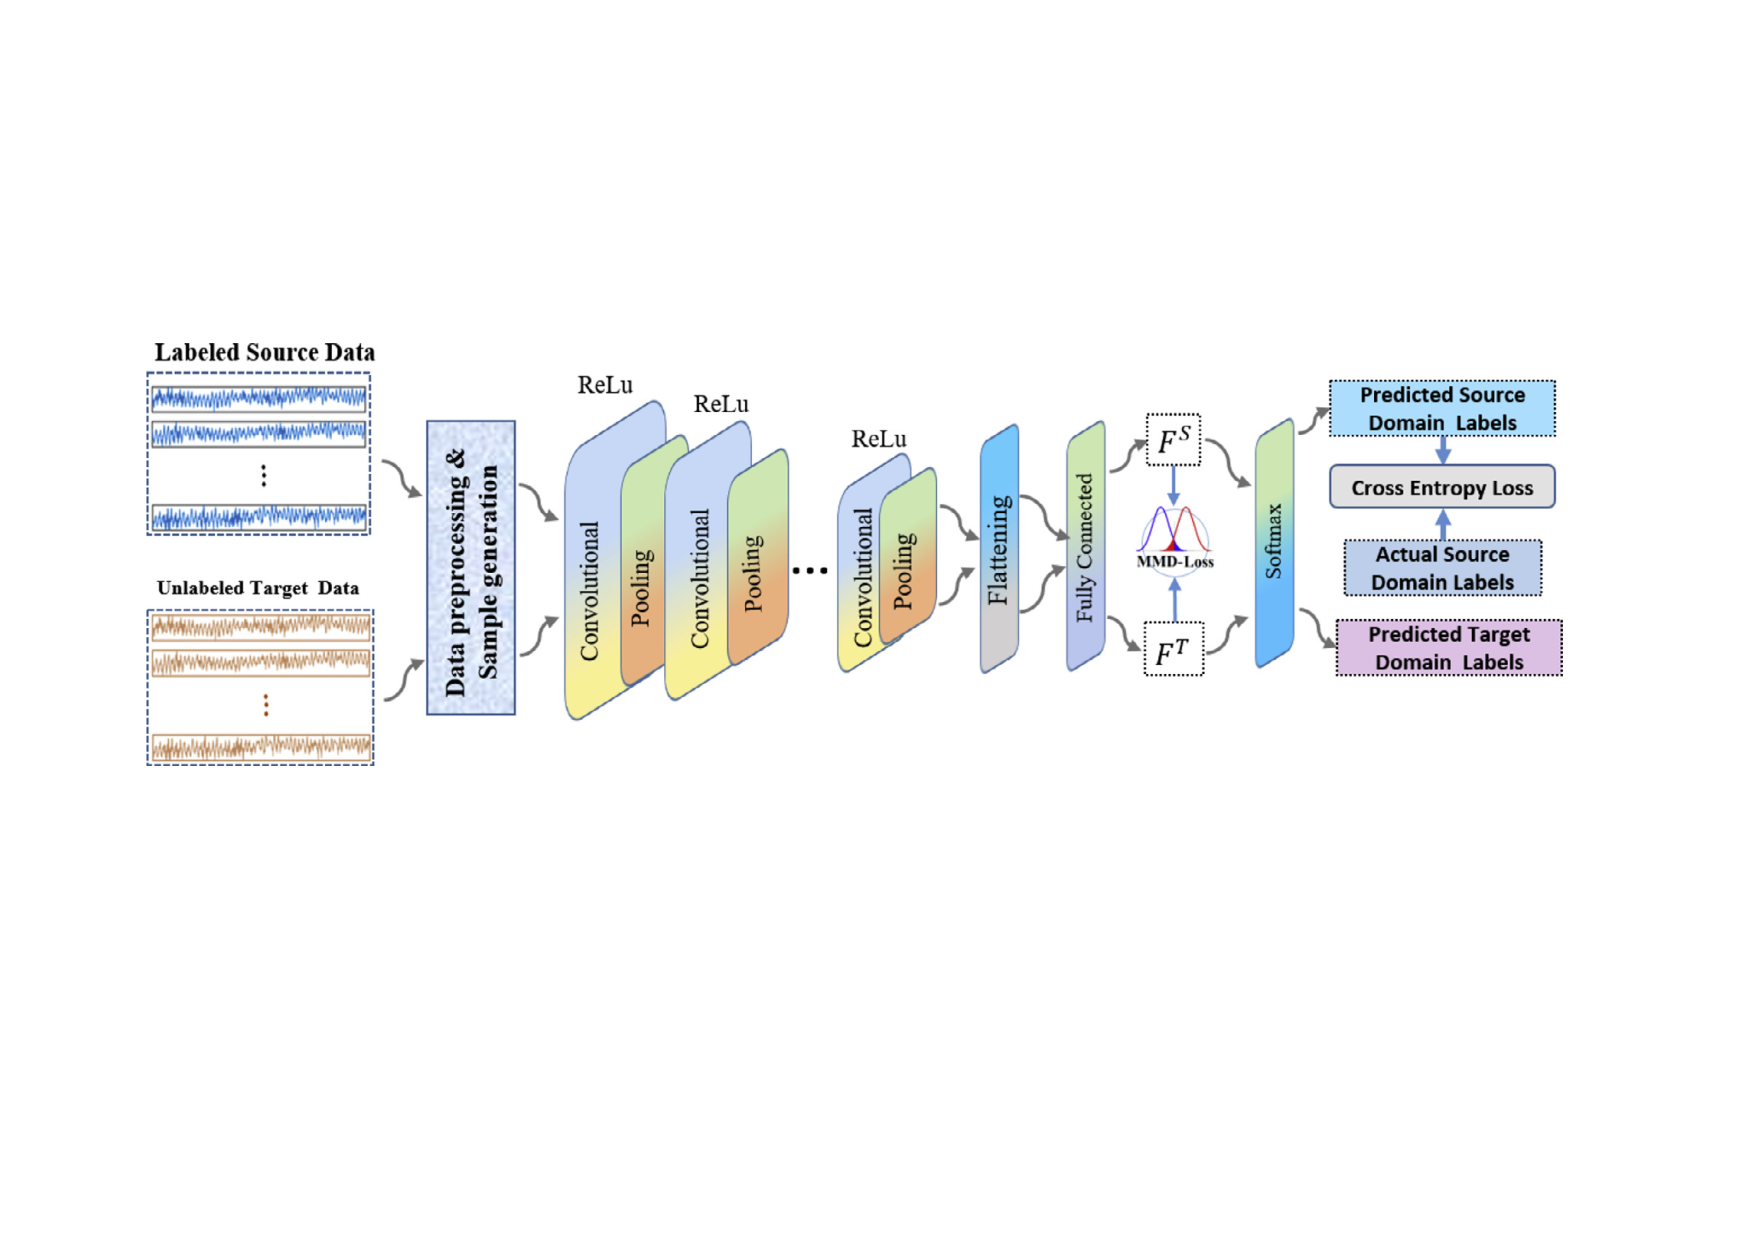
\includegraphics[width=1\textwidth]{models_state_of_the_art/Azamfar_model.pdf}
  \caption{Architecture proposed by Azamfar et al \cite{AZAMFAR2020103932}}
  \label{fig:Azamfar_model}
\end{figure}


\subsection{Deep Domain Adaption based on MMD-Loss and PD Alignment}
Pandhare et al \cite{Pandhare2021} proposed a deep learning-based domain adaption approach for PHM of BSDs, using a MMD-loss and PD alignment. A similar test rig, as the one presented by Azamfar et al \cite{AZAMFAR2020103932}, was used by Pandhare et al to evaluate the proposed models. In total, five accelerometers were mounted in the test bed. Two triaxial ones were placed close to the BSD nut, which seems a promising position to represent the signature of a ball screw preload level. Three single-axial ones were mounted at the bottom and top attachments of the BSD shaft and on top of the load carried by the BSD nut. The last three sensor positions are more suitable and practical installation. Identical to Azamfar et al \cite{AZAMFAR2020103932} nine combinations of degradation classes of BSD and guideways were defined. The domain discrepancy between datasets generated with differently mounted sensors should be reduced by the domain adaption approach of the proposed model. The work tries to find an indirect sensing method to make PHM on BSDs independent of impractical sensor locations. The proposed model architecture is presented in fig. \ref{fig:Pandhare_model} and contains a feature extractor of two convolutional and max pooling layers and a consecutive classifier. The proposed model training includes three losses. Again, a source CE-loss is used to improve the classification performance on the source domain data. The MMD loss reduces the marginal distribution mismatch between the domains. The PD alignment reduces the conditional distribution discrepancy of the domains. This is done by matching source and target samples with equal class label and reducing their L2-distance: 

\begin{equation}
    L_{p} = \frac{1}{n_{p}}\sum_{k=1}^{n_{p}}|h_{k}^{p,s}-h_{k}^{p,t}|_{2}, 
\end{equation}
where $h_{k}^{p,s}$ and $h_{k}^{p,t}$ are the k-th source and target domain samples and $n_{p}$ is subspace of the labeled samples from source and target. 

\begin{figure}[H]
  \centering
  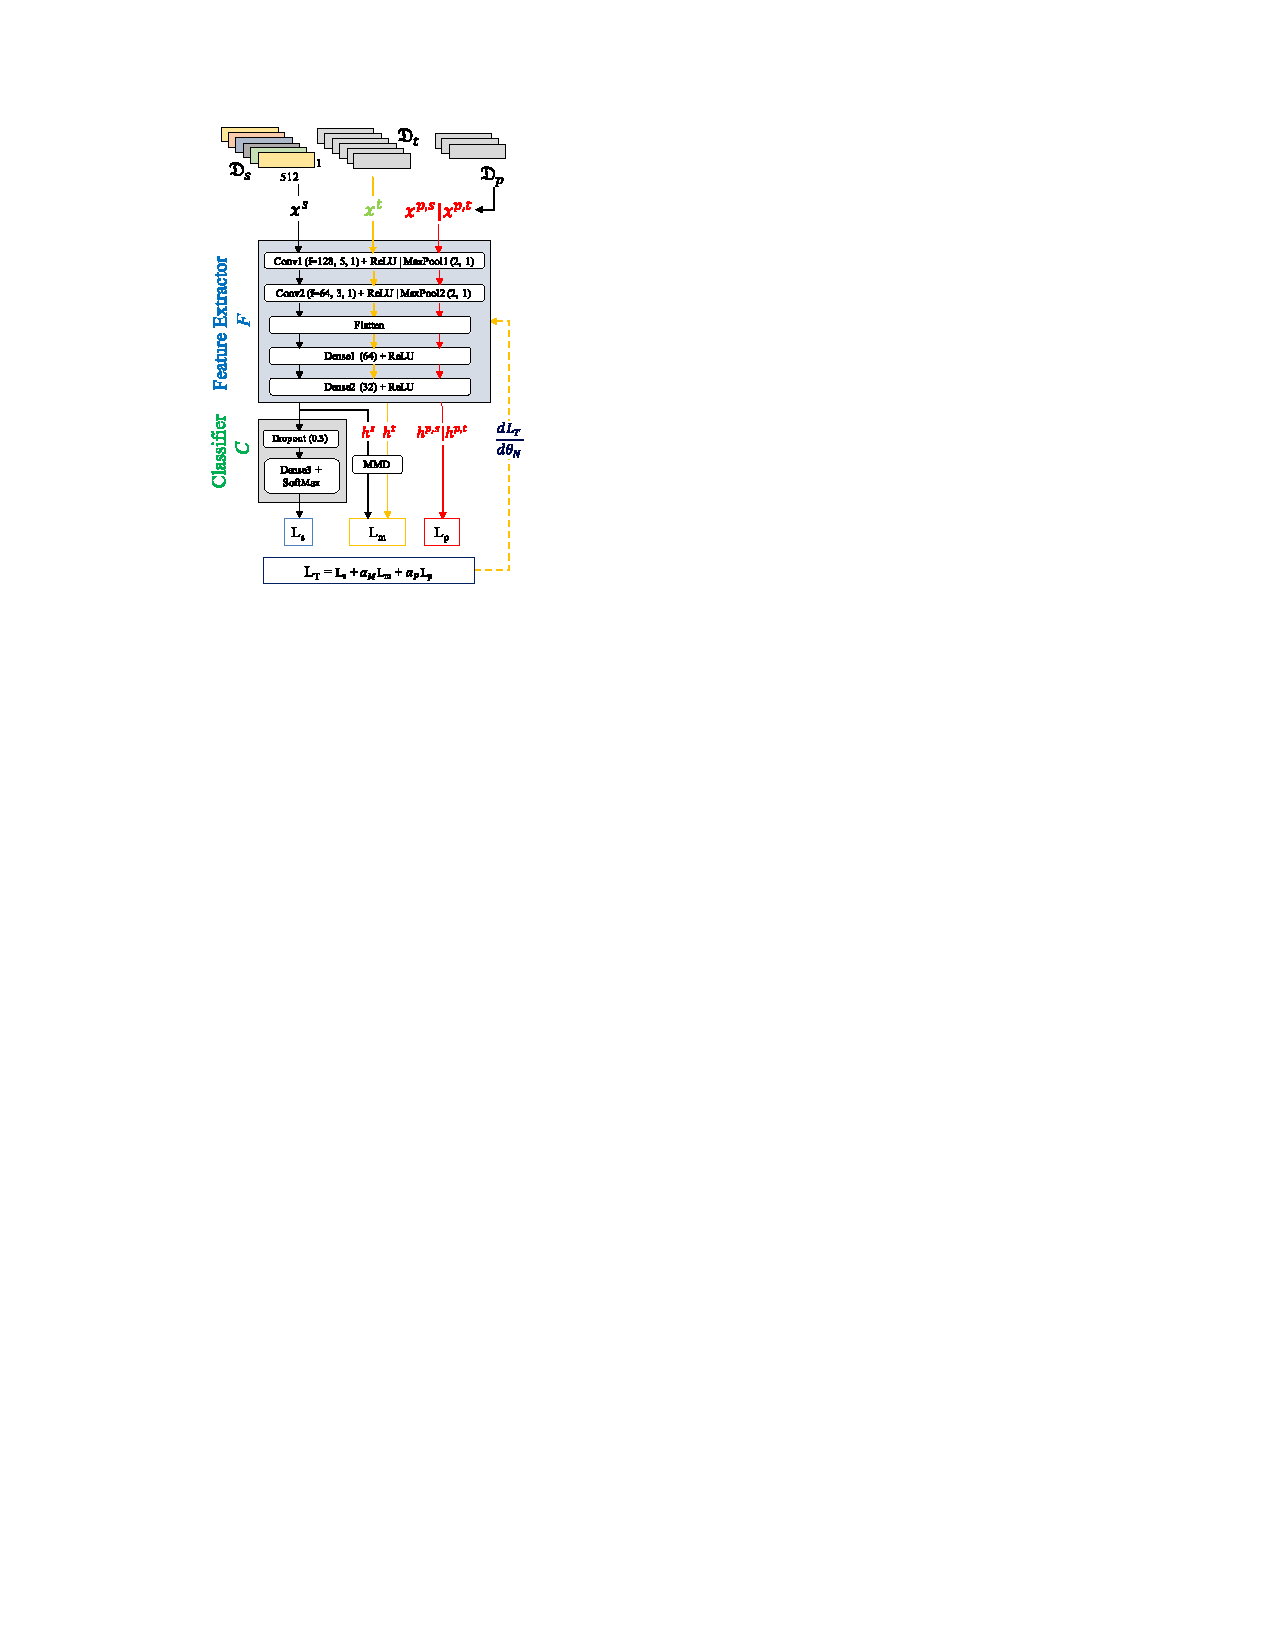
\includegraphics[width=.6\textwidth]{models_state_of_the_art/Pandhare_model.pdf}
  \caption{Architecture proposed by Pandhare et al \cite{Pandhare2021}}
  \label{fig:Pandhare_model}
\end{figure}

\section{Computer Vision Applications which Reduce the Domain Discrepancy in the Feature Extractor}
Most domain adaption approaches reduce the domain discrepancy in task-specific layers but use a shared feature extractor backbone across all domains. In the following two computer vision models are presented, which reduce the domain shift in early layers of the feature extractor. Often the computer vision community offers advanced solution for complex research questions, which were not intensively evaluated in real-world scenarios. For the PHM of BSDs such solutions can be taken as inspiration.

\subsection{Domain Conditioned Adaption Network}
Li et al \cite{li2020} propose a domain conditioned adaption network (DCAN), which contains two separate modules to reduce the domain discrepancy. After each task-specific layer a domain conditioned feature correction block estimates and reduces the domain discrepancy based on the MMD metric. In the CNN backbone an attention module regulates the extraction of domain-specific and -independent features. The proportions of domain-specific and -independent features can be learned to decrease the domain discrepancy. Fig. \ref{fig:DCAN_model} visualizes the domain adaption modules in the DCAN model.

\subsubsection{Domain Conditioned Channel Attention Mechanism}
ResNet is used as backbone network, which allows an easy implementation of the domain conditioned channel attention module in its residual block. In the latent feature maps the processed images are represented as $\pmb{X}_{t} = [X^{1}_{t},...,X^{C}_{t}] \in \mathbb{R}^{HxWxC}$, where H and W are the spatial dimension and C the number of image channels. First, a channel-wise global average pooling layer is applied, which reduces the images to  $\pmb{g}_{t} = [g^{1}_{t},...,g^{C}_{t}] \in \mathbb{R}^{1x1xC}$. Afterwards, the data is split depending on its domain and passed through different fully connected layers. The upper flow is used for target and the lower flow for source domain samples. The two different source and target domain routes share parameters. For both domains, an attention mechanism is trained jointly to learn to activate different channels in the domain samples. This allows extracting more enriched domain-specific features. In the fully connected layers the dimension is first reduced with a ratio ${1x1x\frac{C}{r}}$ and later reconstructed to its original size ${1x1xC}$. ReLU and Sigmoid functions are applied. The domain-wise feature selection is achieved by weighting the channels of the feature representations $\pmb{X}_{s}$ and $\pmb{X}_{t}$ with the channel attention vectors $\pmb{v}_{s}$ and $\pmb{v}_{t}$ calculated by the domain conditioned channel attention module:

\begin{equation}
    \begin{aligned}
        &\pmb{\tilde{X}}_{s} = \pmb{v}_{s} \odot \pmb{X}_{s} = [v_{s}^{1} \cdot X_{s}^{1}, ..., v_{s}^{C} \cdot X_{s}^{C}]\\
        &\pmb{\tilde{X}}_{t} = \pmb{v}_{t} \odot \pmb{X}_{t} = [v_{t}^{1} \cdot X_{t}^{1}, ..., v_{t}^{C} \cdot X_{t}^{C}].
    \end{aligned}
\end{equation}

The domain conditioned channel attention module allows the model to independently learn the importance of each channel for the classification of source and target domain samples \cite{li2020}.


\subsubsection{Domain Conditioned Feature Correction}
The data simultaneously passes through the regular network and the feature correction block, which consist of FC and ReLU blocks. The feature correction block estimates the domain discrepancy in the feature representation of the task-specific layer:
\begin{equation}
    \Delta H_{l}(x_{t}) = H_{l}(x_{s}) - H_{l}(x_{t}),
\end{equation}
where $H_{l}(x_{s})$ and $H_{l}(x_{t})$ are the feature representations of the source and target domain samples in the task-specific layer l. $\pmb{x}_{s}$ and $\pmb{x}_{t}$ are the source and target domain samples. The feature representation of the target domain samples is corrected as following:

\begin{equation}
    \hat{H}_{l}(x_{t}) = H_{l}(x_{t}) + \Delta H_{l}(x_{t}).
\end{equation}

The discrepancy between the regular feature representation of source domain samples $H_{l}(x_{s})$ and the corrected feature representation of the target domain samples $\hat{H}_{l}(x_{t})$ is measured by the MMD-loss in several layers:

\begin{equation}
    L_{M}^{l} = |\frac{1}{n_s} \sum_{i=1}^{n_{s}} \phi(H_{l}(x_{si}) - \frac{1}{n_t} \sum_{i=1}^{n_{t}} \phi(\hat{H}_{l}(x_{ti}))|_{H_{\kappa}}^{2}, 
\end{equation}
where $H_{\kappa}$ is the reproducing kernel Hilbert space (RKHS), $\kappa$ the characteristic kernel and $\phi$ the corresponding feature map. The number of source and target samples is defined by $n_{s}$ and $n_{t}$. To avoid the over-transfer of noise and irrelevant information between source and target, the model is enforced to keep the source data constant when passing through the feature correction blocks \cite{li2020}.

\begin{figure}[H]
  \centering
  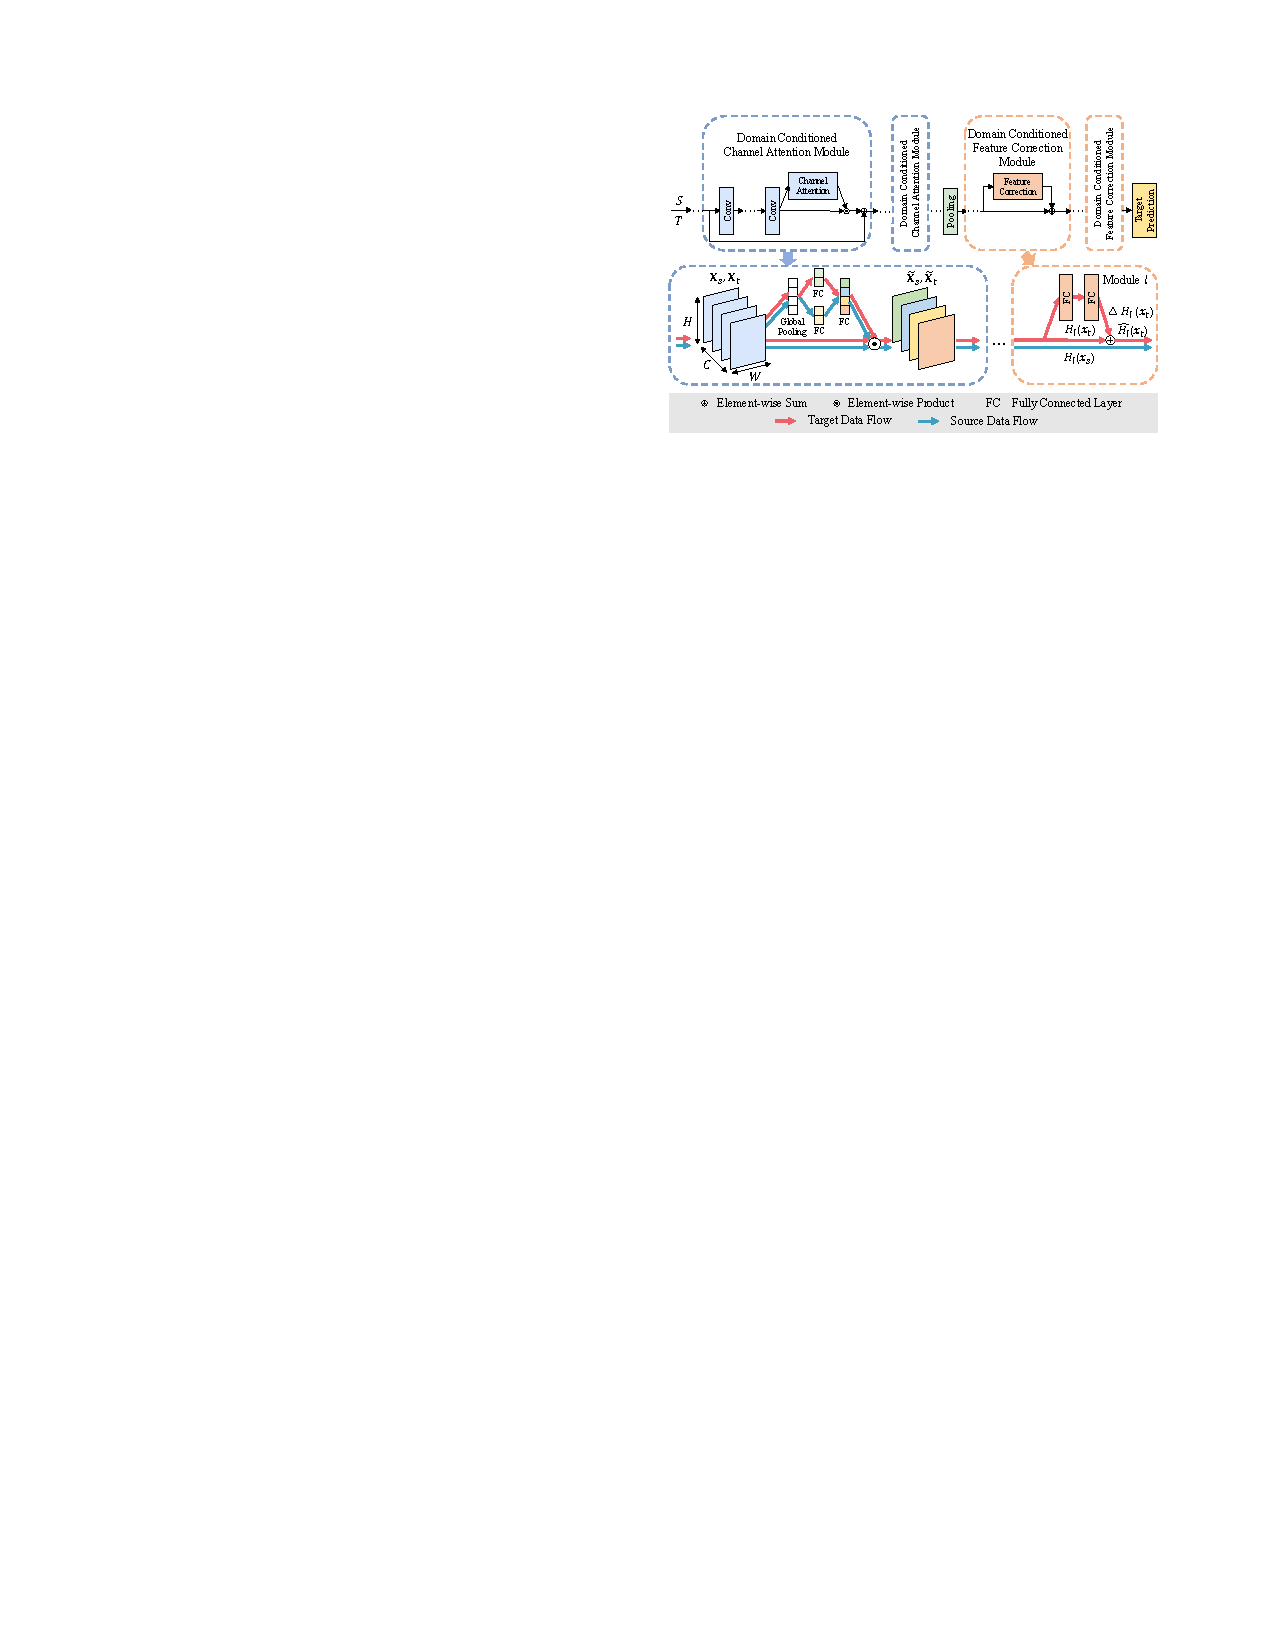
\includegraphics[width=1\textwidth]{models_state_of_the_art/DCAN_model.pdf}
  \caption{DCAN architecture proposed by Li et al \cite{li2020}}
  \label{fig:DCAN_model}
\end{figure}

\subsection{Feature Reconstruction of Domain Shift Affected Layers}
Aljundi et al \cite{Aljundi2016} present a method, which analyzes the output of each convolutional layer for domain shift effects. The goal is to find the layers which suffer most from those effects. By reconstructing them, the new target sample outputs should become more similar to the response given for the source samples. In a first step, the domain shift effects with respect to each layer is measured:
\begin{equation}
    B^{*} = argmin_{B} \{ \sum_{i=1}^{n}( y_{i}-\beta_{0}-\sum_{j=1}^{p}x_{i,j}\beta_{j})^{2} + \lambda \sum_{j=1}^{p}|\Delta_{j}^{KL}\cdot \beta_{j}| \}
\end{equation}
where y is the response, x the output of the various layers, $\beta_{0}$ the residual, $B = \{\beta_{j}\}$ the estimated coefficients for each layer, n the number of
source samples, p the number of layers, $\lambda$ a tuning parameter to punish the value of the coefficients and $\Delta_{j}^{KL}$ the KL divergence measured between the source and target data representation in each layer. When a layer's coefficient is big, it is considered as good (small domain shift effects) and otherwise as bad (big domain shift effects). The optimization is solved by using the coordinate descent method. Afterwards, linear regression is applied to predict new coefficients for the good layers to replace the output of the bad ones. The reconstructed layer outputs are then passed to the subsequent layers. Aljundi et al identified that especially the early layers of the feature extractor are relevant to counteract the domain shift \cite{Aljundi2016}.